\begin{figure}[H]
    \centering
    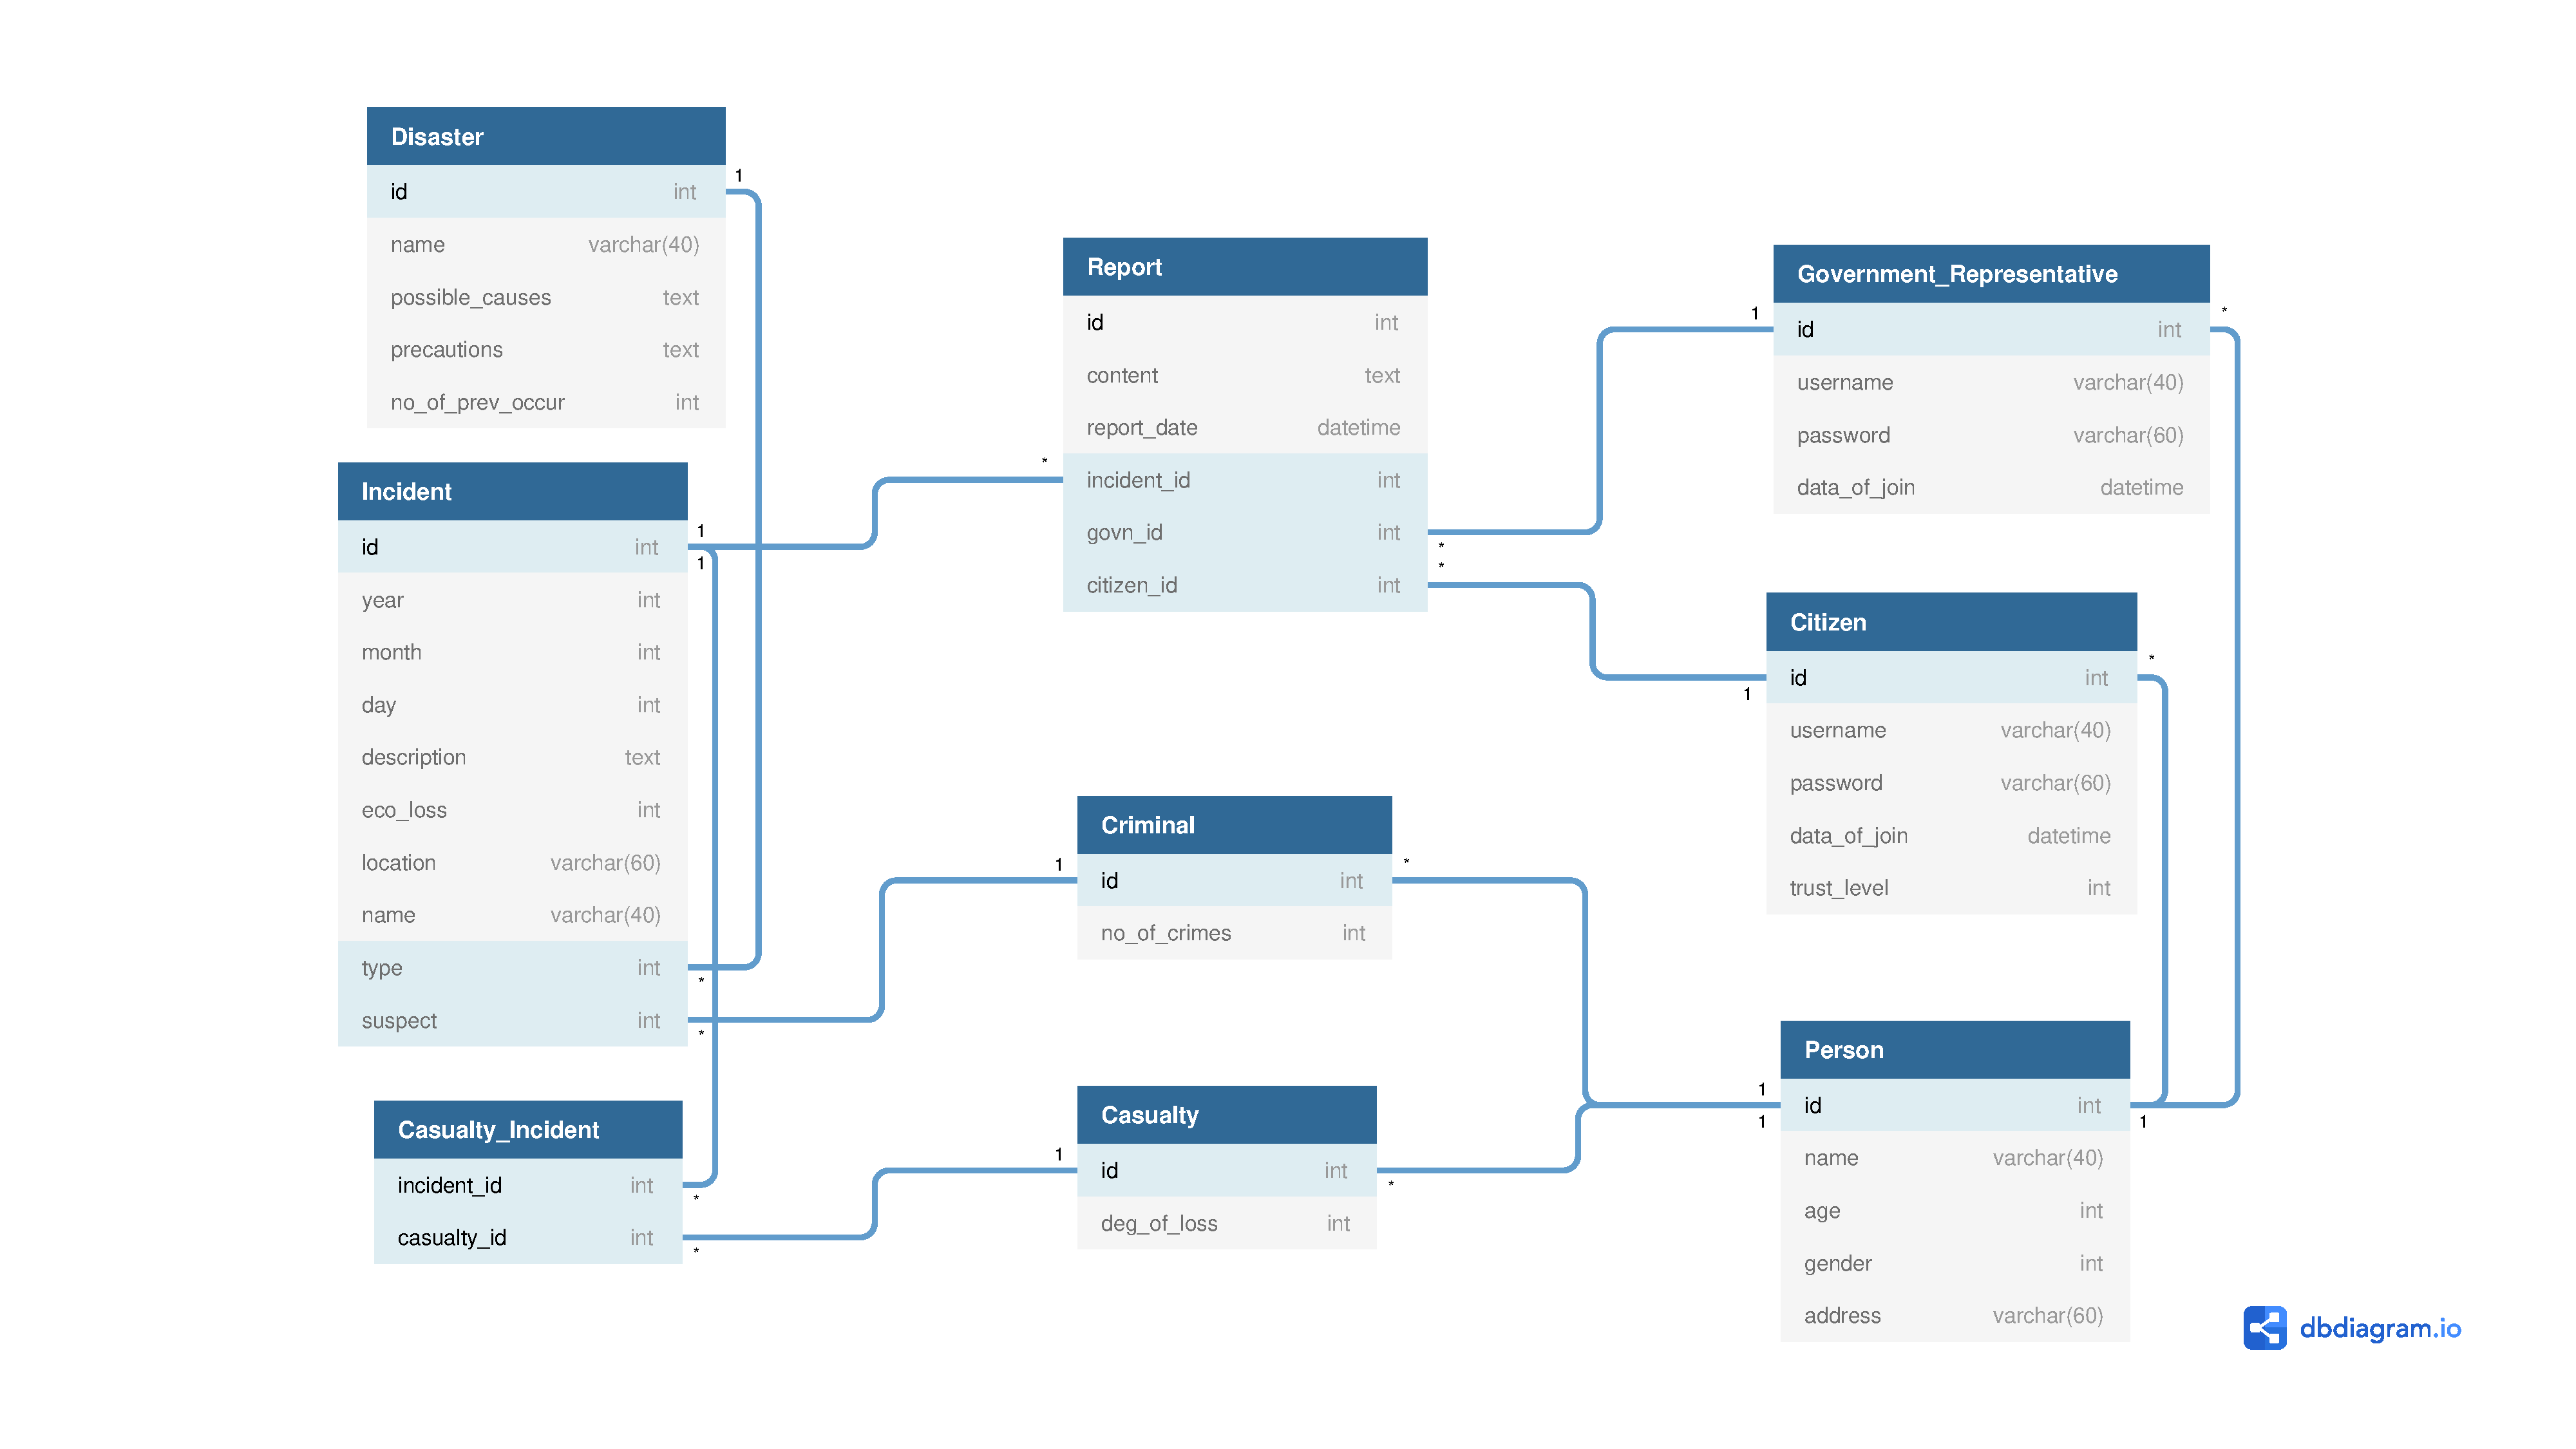
\includegraphics[width=\textwidth]{images/schema.pdf}
    \caption{Database Schema}
    \label{fig:schema}
\end{figure}

\subsection{Schema Illustration}
The chosen system consists of a database that stores \emph{natural} and \emph{man-made} \emph{disasters} for creating an \emph{incident report website}. The database consists of $9$ relations, which are described as follows :
\begin{enumerate}
    \item \textbf{Disaster Relation :} contains the \emph{names} of the main natural and man-made disasters, for example: \emph{the names of famous hurricanes and floods}, and their \emph{causes} and \emph{precautions}.
    \item \textbf{Incident Relation :} contains the information of \emph{specific incidents} of the disasters, like their \emph{dates, locations and descriptions}.
    \item \textbf{Person Relation :} an abstract relation of \emph{all types of persons} that can exist in the database, contains the meta information of any person \emph{(name, age, gender and address)}.
    \item \textbf{Citizen Relation :} contains information of a citizen, \emph{which is the person that can report an incident on the website}. This information includes \emph{username, password, date of join and trust level of the citizen (used to weight the submitted report)}.
    \item \textbf{Government Representative Relation :} contains information of a government representative, \emph{which is the person that can review incident reports on the website}. This information includes \emph{username, password and date of join}.
    \item \textbf{Casualty Relation :} contains the information of a certain casualty in an incident, \emph{which is basically the degree of loss}.
    \item \textbf{Criminal Relation :} contains the information of a certain criminal that committed an incident, \emph{which is basically the number of crimes committed before}.
    \item \textbf{Report Relation :} contains the details of a submitted report, \emph{such as its content and date}. Also, it refers to \emph{a specific incident, a specific citizen that submitted the report and a specific government representative that will review the report.}
    \item \textbf{Casualty\_Incident Relation :} this is basically a relation to specify, \emph{which casualties were in a specific incident (M:N relationship)}.
    
\subsection{Hardware Specifications}
\begin{itemize}
    \item \textbf{Operating System :} Ubuntu $20.04$
    \item \textbf{CPU :} Intel $i5$ $6600k$
    \item \textbf{Utilized RAM Capacity :} $10GB$.
    \item \textbf{Utilized Hard Disk Storage :} $200GB$ \emph{(Current Database Size: 250MB)}.
\end{itemize}
\end{enumerate}